\section{Restricted and free methods: a finite native pilot}
\label{sec:native-priority-method-snapshot}

\subsection{A finite search question, not an increase in world scale}
We compare uniform priorities, adaptive priorities and free code/graph design
under the same declared $L_U=-U$ and $L_C=-U+0.1K$. The institution is optimized;
scientist weights and measurement functions remain fixed. This finite pilot
uses earlier development evidence, without reinterpreting preceding studies.

All methods keep the original four-year/five-founder world, reused development
seed 61001, 103,107-record offline corpus, fixed Qwen3-8B researchers, native
production, resources and catalog durations. Free proposals use the approved
local 35B author and the existing v6 authority over Python, parameters, nodes,
ports, protocols, wires, schedules and bounded processes. They are not confined
to the priority comparator or required to introduce a novel mechanism.
$U$ remains an external abstract-content opinion rather than scientific truth;
$K$ remains collected native activity cost rather than requested expense,
inference compute or welfare. No unpaid-cost, participation or novelty veto
is added to either loss.

Three fresh references precede search: explicit zero priorities, the known
terminal-consolidation version of that system, and the literal related-topic
rule. The first two are visible selectable parents for all methods; the third
is comparison-only. First-minimum reference selection gives the zero system
to U and the terminal system to C. All three yield $L_U=-28.6667$ and $L_T=-36$;
the terminal system has $K=160$ and $L_C=-12.6667$, versus $K=200$ and
$L_C=-8.6667$ for the other two. Its inherited four-unit accounting advantage
is known before search and cannot count as an automatic discovery.

The restricted family varies 53 topic priorities in $[-1,1]$. Minimum original
duration takes precedence, then decreasing priority, then lexical topic.
Every other source, graph, schedule and eligibility field remains literal.
Uniform search uses two uniform proposals. Adaptive search uses one uniform
proposal followed by the existing bounded mutation with initial scale 0.2
and its inverse-square-root schedule. Both start from the exact measured
canonical reference, rather than assigning an old loss to a new anchor.
Their first samples are deliberately paired within each objective/history;
the physically separate evaluations are not independent policy samples.
Free design retains its greedy measured-parent/history feedback procedure.
These are end-to-end method packages, not equal-compute interventions solely
on representational freedom or a benchmark against evolutionary program search.

Two optimizer histories per method/objective use seeds 79011 and 79019, with
two own slots each: 24 own slots plus three references, at most 27 new native
worlds. Generation zero interleaves history, objective and method; generation
one reverses the complete order. Each world has 1,024 scientist HTTP attempts,
900s zero-retry scientist transport and 7,200 safe-point wall seconds. The
fixed content observer permits 6,000 critic POSTs. Free design has 16 proposal
calls per session, initial and actual-request readiness, at most 488 combined
readiness/proposal POSTs and 512 component probes; role loads remain separate.
Shared-host time is not a dedicated throughput measurement.

Known technical nulls consume slots with unknown loss, not a hidden penalty
or refill. Changed bindings or unknown dispatch stop the experiment. At budget
end, selection is the earliest tied complete own submission for each cell,
or none, without reference fallback. Two optimizer seeds do not provide two
independent researcher populations. No unused-condition evaluation belongs
to this pilot.

\subsection{All 24 submitted outcomes and frozen own-only selection}
\label{sec:native-priority-prefix}
The original writer and its supervisor exit normally at November 16, 2026,
14:05 UTC. All 24 own native observations and three references are recorded;
the own-only earliest-tie selections are frozen. At the 14:11 UTC verification,
loss recomputation and literal selection checks agree with those records.
The full original-source paired cold audits, campaign cost closure and paired
all-slot readouts are still running; this terminal snapshot is not that audit.
Table~\ref{tab:native-priority-prefix} retains every submitted slot in order,
not a selected subset: 12 tie and 12 worsen their strong visible reference,
with zero improvements beyond it. There are no generation or execution nulls
in these 24 slots. The earlier dated 15- and 20-slot receipts remain unchanged.

At 14:21 UTC the original chain has subsequently closed: both full native cold
audits and cost exports agree, both all-slot readouts agree, and both all-eight
author/outcome exports agree. A separate guarded visibility export also runs
twice with identical three-file outputs. Every original continuation exits
zero, with no new model calls, candidate repair or native-world restart.
The terminal-only evidence above and this later full closure are distinct
dated records. The final counts and frozen selections do not change.

\begin{table}[t]
\centering\small
\setlength{\tabcolsep}{5pt}
\begin{tabular}{rlllrrr}
\toprule
Slot & Method & $h/g$ & Target & $L_U$ & $L_C$ & $L_T$\\
\midrule
1 & R & 0/0 & U & $-27.67$ & $-7.67$ & $-36$\\
2 & A & 0/0 & U & $-27.67$ & $-7.67$ & $-36$\\
3 & F & 0/0 & U & $-28.67$ & $-8.67$ & $-36$\\
4 & R & 0/0 & C & $-25.67$ & $-9.67$ & $-36$\\
5 & A & 0/0 & C & $-25.67$ & $-9.67$ & $-36$\\
6 & F & 0/0 & C & $-28.67$ & $-12.67$ & $-36$\\
7 & R & 1/0 & U & $-28.67$ & $-8.67$ & $-36$\\
8 & A & 1/0 & U & $-28.67$ & $-8.67$ & $-36$\\
9 & F & 1/0 & U & $-28.67$ & $-8.67$ & $-36$\\
10 & R & 1/0 & C & $-25.67$ & $-9.67$ & $-36$\\
11 & A & 1/0 & C & $-25.67$ & $-9.67$ & $-36$\\
12 & F & 1/0 & C & $-28.67$ & $-12.67$ & $-36$\\
13 & F & 1/1 & C & $-28.67$ & $-12.67$ & $-36$\\
14 & A & 1/1 & C & $-28.33$ & $-12.33$ & $-36$\\
15 & R & 1/1 & C & $-28.67$ & $-12.67$ & $-36$\\
16 & F & 1/1 & U & $-28.67$ & $-8.67$ & $-36$\\
17 & A & 1/1 & U & $-28.33$ & $-8.33$ & $-36$\\
18 & R & 1/1 & U & $-28.33$ & $-8.33$ & $-36$\\
19 & F & 0/1 & C & $-28.67$ & $-12.67$ & $-36$\\
20 & A & 0/1 & C & $-26.33$ & $-10.33$ & $-36$\\
21 & R & 0/1 & C & $-26.33$ & $-10.33$ & $-36$\\
22 & F & 0/1 & U & $-28.67$ & $-8.67$ & $-36$\\
23 & A & 0/1 & U & $-28.67$ & $-8.67$ & $-36$\\
24 & R & 0/1 & U & $-28.33$ & $-8.33$ & $-36$\\
\bottomrule
\end{tabular}
\caption{All 24 complete own slots at normal writer closure. R denotes uniform
priorities, A adaptive priorities, F free code/graph; $h/g$ is optimizer history
and generation. Lower losses are better. Rounded values are for display only;
literal full-precision observations and feedback are retained. Frozen selection
is summarized separately, not inferred from rounded table ties. Subsequent paired
closure confirms every row. The interface limitation below prevents an
isolated clean method/objective attribution.}
\label{tab:native-priority-prefix}
\end{table}

Across the 12 frozen method/history/objective selections, eight tie and four
worsen the common visible reference; none improves it. Free design ties in all
four cells. Adaptive priorities tie in both U histories; their C losses remain
$7/3$ and $1/3$ worse in histories 0 and 1. Uniform priorities are $1/3$ worse
and tied in U, and $7/3$ worse and tied in C, respectively. Each cell selects
only its own two submissions, without falling back to the stronger reference.
These small, deliberately coupled histories on one reused researcher condition
are not independent populations, confidence intervals or method-superiority
evidence. In particular, the later adaptive U recovery to the reference does
not establish an advantage over free design or uniform search in expectation.

\begin{figure}[t]
\centering
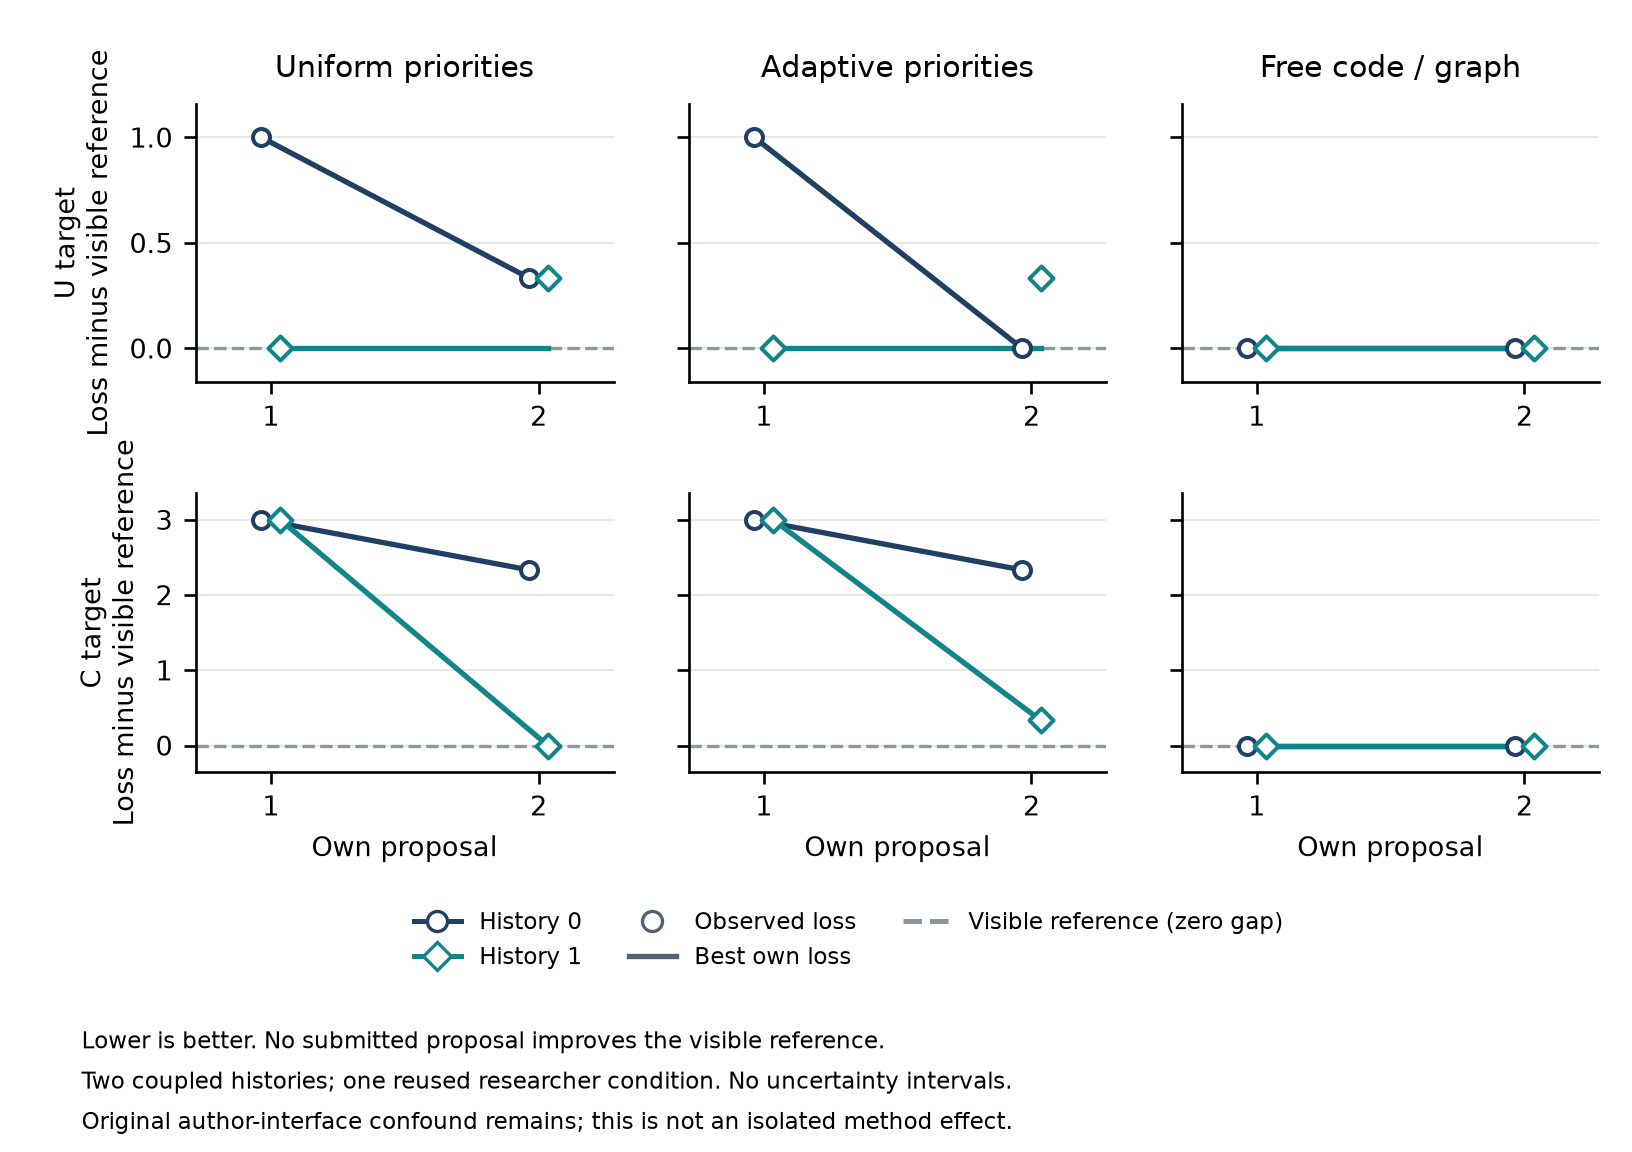
\includegraphics[width=\linewidth]{figures/native-priority-method-v1/method-loss-paths.png}
\caption{All 12 two-proposal optimization paths in the finite native pilot.
Symbols show actual submitted losses; solid lines show best own losses so far.
Gaps are relative to the common visible reference for the assigned objective,
not different retrospectively substituted losses. No proposal improves on that
reference. History 1/U numeric generation one worsens while its own incumbent
remains tied. Small horizontal offsets only separate overlapping symbols.
Both histories reuse the same researcher condition, and first numeric proposals
are paired. The original author-phase confound remains; these are not isolated
method effects, independent-population intervals or corrected-inventor results.}
\label{fig:native-priority-method-paths}
\end{figure}

The initial U numeric proposals change two founders' actual topics while
preserving durations/deadlines; their complete 186 scientist inputs differ
from the reference's 179, and assigned loss worsens by one. This is operated
parameter variation, not an unused coordinate. The paired first samples do
not constitute an adaptive step. In history 1/C, adaptive generation one
improves its previous own loss by $8/3$ but remains $1/3$ worse than the known
terminal reference. Uniform generation one improves its previous own loss
by three and ties that reference. Own-to-own recovery and a best-known gain
are different, and these observations establish no adaptive advantage.

\paragraph{Two literal edits with different internal but inert outside effects.}
Free history 1/U/generation zero writes a feature extractor that adds one to
an internal base-utility feature. All four annual features/scores change from
zero to one, but the native accept-all control does not use that feature as
the external content measurement. Native decision identities/final scores,
all 179 complete scientist inputs and literal response choices remain equal
to the parent. Complete paper records still have different submission times;
this is not whole-record or world byte identity. Assigned loss ties the parent.

Free history 1/C/generation one instead writes an actual new catalog-agenda
function. It keeps minimum duration first and replaces parameter priorities
with nine hardcoded biases over real catalog topics, including artificial
intelligence and deep learning. Fourteen recorded actions contain one source
write, eleven reads, seven duplicate unchanged reads and explicit finish.
It adds no node, wire or schedule. On all 18 actually logged eligible actor/year
inputs, its ranking selects the same direction and duration as the lexical
parent: preferred tied choices already coincide, or a shorter duration wins.
All 18 logged agenda records differ only in reason text; all 179 complete
scientist inputs and literal choices match the reference, while full provider
envelopes differ. $U$, $K$ and all three losses tie. The function was generated
and executed, but this observed-path edit is not a useful new institution or
evidence of equivalence on unobserved inputs.

\subsection{A real author-interface confound, not a repaired result}
\label{sec:native-author-visibility}
Source and saved-request inspection identify an interface inconsistency.
The active V45 renderer supplies the whole compact JSON document when it
fits 65,536 UTF-8 bytes. Its inherited V44 phase function independently uses
spaced JSON against the same cap. V45 then replaces only the displayed
visibility flag, after phase selection. A fully supplied document can therefore
remain in the general tool phase after three inspection attempts rather
than reaching the declared implementation checkpoint. The counter records
attempts, not only successful reads; the three initial boundary inspections
in these examples all succeed.

\begin{table}[t]
\centering\small
\setlength{\tabcolsep}{5pt}
\begin{tabular}{lrrl}
\toprule
Actual complete document & Supplied bytes & Spaced bytes & Phase after 3 reads\\
\midrule
Zero-priority U parent & 61,892 & 65,479 & Implementation\\
Terminal C parent & 62,755 & 66,342 & General\\
U after feature-source write & 62,032 & 65,619 & General\\
\bottomrule
\end{tabular}
\caption{Different serializations, same numeric cap. All three actual native
documents fit the supplied-body limit. The 140-byte U edit crosses only the
legacy spaced-JSON boundary, changing its tool-phase schedule despite continued
full visibility. This is an interface confound, not native loss corruption.}
\label{tab:native-author-visibility}
\end{table}

This defect must not be projected onto every earlier study. A separate
retrospective check covers all eight completed author sessions and 101 original
requests in the preceding source-information pilot. Every request supplies
the whole document; actual sizes range from 60,210 to 60,885 compact bytes
and 63,690 to 64,365 spaced bytes, fitting both limits. No instance of this
specific visibility/phase mismatch is observed there. Its original seven
complete outcomes, one native null and four tied selections are unchanged.
This scoped absence is not a certificate that its entire interface is bug-free
or proof of model comprehension. It does not extend to uninspected studies.

Three complete initial sessions supply 33 saved backend requests, including
14 affected general-phase calls. The subsequent C/generation-one session has
nine further affected calls. Exact loss arithmetic and measurement definitions
are present in the first 33 inspected wires; in particular, institution-written
\code{final\_score} is not an input to external $U$. Their observed prompt counts
32,070--37,382 fit the reserved 8,192 output tokens within 65,536, and replies
end in stop. These diagnostics do not establish model understanding or absence
of backend truncation. Read bytes were not silently lost. Fourteen-action
finishes at the three-call submission reserve must not be called freely chosen
early strategic stops. Actual own scalar feedback reaches the next-generation
backend request, which proves delivery rather than useful use.

The four original scientific/analysis sources remain pinned and unchanged.
Native measurements, candidates, nulls and costs are not rewritten, refilled
or converted to failures because of this defect. However, parent and edited
document sizes also changed the allowed-tool schedule. This old pipeline is
therefore source-specific exploratory evidence, not a clean isolated comparison
of objectives, intrinsic model ability or numerical versus free design.
No conclusion is drawn about whether an unobserved corrected proposal would
have improved the loss.

\paragraph{Prospective repair and its narrower evidence.}
The corrected renderer determines actual document inclusion before computing
the workflow and passes a source-owned boolean into phase selection. Legacy
V44 behavior without that override, the byte cap, the 16-call budget and the
three-call submission reserve are preserved. This restores the declared
technical interface without mandatory edits or a novelty/merit constraint.
The new context contract is explicitly named
\code{matched-bounded-author-64k-v2-literal-visibility}; older model certificates
cannot authorize the changed source.

Complete native document fixtures reproduce two pre-fix failures. The fixed
author source passes 87 light/scripted boundary, wire and replay checks with
one unavailable optional archive skipped and one explicit historical case
deselected. A further source-contract preparation stop is retained, rather
than bypassed. Prospective routes then bind the designer-only correction as
an explicit Git-versioned adapter, leaving the original byte guard and its
exclusions unchanged; 43 scoped light cases include rejection of injected
author/scientist/executor drift. The older free-topic driver keeps its narrower
contract and is tested against its immutable original bytes. These are software
and static bindings, not new real-model readiness, full native/public execution
or an observed benefit from the repair. None is established by these checks.

A subsequent complete public/native software check at source \code{adfd6b94}
passes in 1,245.16 shared-host seconds. It uses the actual SDK, executor,
checkpoints and paired cold/cost/readouts, including 27 development, two
upstream-fixture and 18 fixed-evaluation native worlds. Its HTTP responses,
corpus and orchestration are explicitly scripted; software seeds 43003/43011
do not consume reserved scientific conditions. All 30 logical evaluation rows
and 108 contrast rows are retained. This is a real execution-path check, not
real-model readiness, outer subprocess-CLI proof or useful institution search.

\subsection{What remains a scientific question}
All eight proposal sessions have generated with 102 committed proposal steps;
a read-only journal projection finds 45 instances of the specific phase
mismatch and no different loss views. These are repeated steps within eight
sessions, not 102 independent author trials. All eight native outcomes are now
recorded, but the original all-eight author/outcome join and the guarded paired
visibility export are not complete at the terminal snapshot; their later
14:21 UTC closure confirms all eight parent-matching input paths. Generated edits
and measured improvement remain distinct. For example, the final free U
source emits the same 18 actual project commands despite removing its own
agenda-assignment bookkeeping; its 179 full researcher inputs and literal
choices equal the reference and its loss ties. A self-reported zero counter
does not mean that no researcher acted or that the edit failed to execute.

The final all-eight action summary records five actual source writes in four
changed submissions, four unchanged submissions, 52 duplicate unchanged reads
and explicit finish in all sessions. Every submitted native outcome is complete
and tied with its measured parent; all eight observed full researcher-input
paths match a complete parent path. No node, wire or schedule changes are
submitted. Neither a valid finish nor five successful writes establish useful
institution invention. The specific phase confound remains, rather than being
erased by full audit closure.

\paragraph{Actual inference accounting, not an equal-compute experiment.}
The original full campaign records 4,888 complete researcher responses, all
with reported usage: 7,392,125 prompt tokens and 442,516 output tokens; no saved
researcher input lacks a committed reply. Separate physical content-critic
requests number 213. The author performs 256 readiness and 102 proposal POSTs,
with 17 designer-load and 27 scientist-load records kept separate. The writer
takes 35,144.9 seconds on a shared host, not dedicated model throughput, energy,
money or the sum of nested call durations. These totals include references and
calibration, not just the 24 optimization observations. Their non-overlapping
role counts do not imply equal measured compute across methods.

Further inference should not automatically enlarge a flat pilot. A corrective finite study
requires appropriate exact-source native verification and fresh real readiness
before dispatch, with a frozen protocol and no failed-slot refill. Separately,
unused-condition evaluation of old selected policies would answer their transfer
question, not validate the corrected inventor. No such evaluation is completed
by this snapshot. Important differentiated findings, adequate independent
evidence and a final main-track submission judgment remain open.

\begingroup\raggedright
Literal sources and dated evidence are retained under scientific commit
\code{705b5259}; prospective author checks use \code{195739f6}, and scoped
source-binding tests use \code{1e3b114b}. All 24 literal outcomes and frozen
selection checks are in
\path{research/results/native-priority-method-terminal-snapshot-v1.json}.
The later paired cold/cost/readout/author/visibility closure is retained in
\path{research/results/native-priority-method-comparison-closed-v1.json}, with
compressed literal reports and their original-file hashes.
The earlier 15-slot prefix is in
\path{research/results/native-priority-first-three-second-generation-outcomes-v1.json};
the defect and original failures are in
\path{research/results/native-author-workflow-visibility-correction-v1.json}
and the additional bindings in
\path{research/results/native-author-context-source-binding-v2.json}.
The separate successful public/native software verification is in
\path{research/results/native-priority-corrected-public-native-qa-v1.json}.
The earlier pilot's complete author-side scope check is in
\path{research/results/native-consumer-source-visibility-diagnostic-v1.json}.
Normal writer completion is not the paired original cold audit, corrected-model
proof or a publication-ready differentiated finding.
\par\endgroup
\FloatBarrier
